\chapter{Адаптивная стоимостная модель}\label{ch:ch2}
\section{Введение}\label{sec:ch2/sec1}
В области систем управления базами данных общеизвестно, что для одного и того же запроса может существовать несколько планов выполнения. Чтобы решить задачу выбора плана исполнения, СУБД используют сложные алгоритмы и методы оптимизации, подбирая наиболее эффективный план для заданного запроса. Эти процедуры в первую очередь ориентированы на оценку времени выполнения, поскольку основная цель — минимизация времени исполнения запроса. Для достижения этой цели большинство современных СУБД применяют стоимостную модель, которая оценивает время выполнения планов-кандидатов на основе собранной статистики и базовых предположений о производительности системы. Такой подход позволяет оценивать любой сгенерированный план, включая ранее не встречавшиеся.

Стоимостной оптимизатор опирается на три основных компонента: оценку количества результирующих строк (кардинальности) на каждом узле и в плане в целом, параметры стоимостной модели и алгоритм перебора планов. Каждому узлу плана назначается стоимость: чем она выше, тем большее время выполнения предсказывает модель. Используя эти компоненты, СУБД стремятся выбрать наиболее эффективный план, повышая общую производительность и надёжность системы. Однако у такого подхода есть существенные недостатки: при оценке стоимости сложных запросов с многочисленными соединениями возможны ошибки, из-за которых время выполнения запроса для разных планов может отличаться на \textbf{несколько порядков}. В данной работе рассматривается новый подход к настройке параметров стоимостной модели, при этом проблема оценки кардинальностей и алгоритмы перебора планов остаются за рамками рассмотрения.

В последние годы предложены обучаемые оптимизаторы, использующие методы машинного обучения и опирающиеся на опыт прошлых выполнений запросов. Такой подход частично смягчает проблемы стоимостных оптимизаторов, поскольку обучаемый оптимизатор способен извлекать закономерности из ранее наблюдавшихся сложных примеров. Однако обучаемые оптимизаторы не лишены недостатков: такие модели часто требуют длительного обучения и значительного объёма данных, усложняют эксплуатацию в высоконагруженной среде из-за дополнительной инженерной нагрузки, а также могут частично игнорировать экспертные знания и эвристики, накопленные за десятилетия разработки СУБД.

Традиционно администратор БД (DBA) настраивает параметры стоимостной модели вручную. Подбор наилучших значений требует глубокого понимания структуры базы данных, характеристик нагрузки и системных ресурсов. Неверная настройка параметров стоимости может приводить к неоптимальным планам и ухудшению производительности. Более того, параметры часто приходится периодически корректировать, чтобы адаптироваться к изменениям нагрузки, данных и характеристик системы. Поэтому настройка и выбор оптимальных параметров сами по себе представляют значительную проблему.

Альтернативный подход использует калибровочную нагрузку: под конкретные данные и схему формируются синтетические запросы, далее они выполняются, и по ним собирается статистика исполнения. Затем решается система линейных уравнений, где неизвестными являются параметры стоимостной модели, а коэффициентами при этих параметрах служат измеренные объёмы обработанных кортежей, число выполненных операций, количество индексных обращений и объём обработанных страниц. К недостаткам метода относятся необходимость запуска синтетической калибровочной нагрузки помимо реальной, потребность в периодической перекалибровке, а также риск того, что синтетическая нагрузка приведёт к неточным оценкам параметров для реальной рабочей нагрузки.

В данной работе предлагается \textbf{адаптивная стоимостная модель (Adaptive Cost Model, ACM)} как подход к настройке параметров стоимостной модели, который снижает потребность в ручной настройке и устраняет необходимость калибровки на синтетической нагрузке за счёт использования статистики предыдущих запусков и лёгких моделей машинного обучения. Подход позволяет выполнять онлайн настройку параметров и адаптироваться к изменению рабочей нагрузки без выполнения калибровочных запросов, снижая дополнительную нагрузку на СУБД и позволяя администраторам баз данных сосредоточиться на более критических задачах. Система включает два компонента: модель для оценки параметров, связанных с производительностью CPU, и модель для оценки параметров, связанных с дисковой подсистемой.

\section{Постановка задачи}

Большинство открытых стоимостных СУБД с «bottom-up» оптимизацией используют стоимостную модель на основе пяти ключевых параметров (например, PostgreSQL, MySQL, openGauss). В PostgreSQL и openGauss эти параметры следующие:

\begin{enumerate}
    \item \(cpu\_tuple\_cost\) — Задаёт оценку планировщика стоимости обработки каждой строки во время выполнения запроса. Значение по умолчанию 0.01;
    \item \(cpu\_index\_tuple\_cost\) — Задаёт оценку планировщика стоимости обработки каждой записи индекса при индексном сканировании. Значение по умолчанию 0.005;
    \item \(cpu\_operator\_cost\) — Задаёт оценку планировщика стоимости выполнения каждого оператора или функции в запросе. Значение по умолчанию 0.0025;
    \item \(seq\_page\_cost\) — Задаёт оценку планировщика стоимости чтения дисковой страницы, когда чтения происходят последовательно, серией. Значение по умолчанию 1.0;
    \item \(random\_page\_cost\) — Задаёт оценку планировщика стоимости чтения дисковой страницы при непоследовательном доступе. Значение по умолчанию 4.0.
\end{enumerate}

Помимо этих параметров существуют и другие, однако именно эти пять являются основными для оптимизации запросов. Стоимость всего плана вычисляется как сумма стоимостей операторов в плане. Стоимость операторов выражается линейной комбинацией базовых параметров (релевантные стоимости GUC-параметры выступают числовыми константами) и переменных величин — таких как число блоков данных, считанных с диска, и другие.

Стоимость выполнения оператора оценивается как линейная комбинация параметров стоимостной модели и измеримых объёмов работы:
\begin{equation}
    Cost_{operator}=c_t \cdot n_t+c_o \cdot n_o+c_s \cdot n_s+c_i \cdot n_i+c_r \cdot n_r,
\end{equation}
где:
\begin{itemize}
    \item \(c_t\) , параметр \(cpu\_tuple\_cost\), стоимость обработки одной строки,
    \item \(n_t\) , оценка числа обработанных строк (кортежей),
    \item \(c_o\) , параметр \(cpu\_operator\_cost\), стоимость выполнения одной операции или функции,
    \item \(n_o\) , оценка числа выполненных операций или вызовов функций,
    \item \(c_s\) , параметр \(seq\_page\_cost\), стоимость чтения одной страницы при последовательном доступе,
    \item \(n_s\) , оценка числа страниц, прочитанных последовательно,
    \item \(c_i\) , параметр \(cpu\_index\_tuple\_cost\), стоимость обработки одной записи индекса,
    \item \(n_i\) , оценка числа обработанных записей индекса,
    \item \(c_r\) , параметр \(random\_page\_cost\), стоимость чтения одной страницы при непоследовательном доступе,
    \item \(n_r\) , оценка числа страниц, прочитанных при непоследовательном доступе.
\end{itemize}

\textbf{Пример 1.} Стоимость оператора последовательного сканирования \texttt{SeqScan} (без фильтра):
\[
Cost_{SeqScan}=c_t \cdot n_t+c_s \cdot n_s
\]

\textbf{Пример 2.} Стоимость оператора агрегирования \texttt{Aggregate}:
\[
Cost_{Agg}=c_t \cdot n_t
\]

Точность вычисления стоимости операторов и, как следствие, оптимальность выбранного плана зависят от корректности параметров стоимостной модели. Оптимальные значения этих параметров определяются аппаратной конфигурацией, типом рабочей нагрузки, а также степенью разогрева системы, то есть долей данных, находящихся в буферном кэше.

Главная цель настройки параметров стоимостной модели состоит в повышении согласованности между вычисляемой стоимостью и фактическим временем выполнения оператора. Это позволяет более надёжно сравнивать планы-кандидаты и оценивать ожидаемое время выполнения плана. Таким образом, задача настройки сводится к максимизации корреляции:

\begin{equation}
    corr(cost, time) \rightarrow 1
\end{equation}
где
\begin{itemize}
    \item \(cost\) , стоимость оператора, вычисленная стоимостной моделью,
    \item \(time\) , фактическое время выполнения этого оператора,
\end{itemize}

Корреляция вычисляется по множеству операторов, наблюдаемых в наборе выполнений запросов. При этом требуется, чтобы изменение стоимости отражало изменение времени выполнения, в том числе в относительных величинах.

\section{Метод калибровочных запросов}
В этом разделе описан базовый метод настройки параметров стоимостной модели на основе калибровочных запросов, используемый далее как сравнение для предложенной адаптивной стоимостной модели. Метод опирается на идею из работы \cite{10.1109/ICDE.2013.6544899} и сводит оценку параметров стоимости к решению линейной системы, построенной по измерениям времени и объёмов работы операторов на калибровочных запросах.

\subsection{Общая схема метода}
Рассматривается вектор параметров стоимостной модели
\[
\mathbf{c} =
\left(
\begin{aligned}
&seq\_page\_cost,\; \\
&random\_page\_cost,\; \\
&cpu\_tuple\_cost,\\
&cpu\_index\_tuple\_cost,\; \\ 
&cpu\_operator\_cost
\end{aligned}
\right)^{T}
\]
Для каждого запуска калибровочного запроса \(q_j\) измеряется фактическое время выполнения \(t_j\) и формируется вектор признаков \(\mathbf{n}_j\), отражающий число обработанных кортежей, число индексных обращений, число прочитанных страниц при последовательном и непоследовательном доступе, а также число выполненных элементарных операций. Далее предполагается линейная зависимость вида
\begin{equation}
t_j \approx \mathbf{n}_j \cdot \mathbf{c}.
\end{equation}
Собирая измерения для набора запросов, получаем матричную форму:
\begin{equation}
\mathbf{t} \approx \mathbf{N}\mathbf{c},
\end{equation}

где \(\mathbf{t}\) это вектор измеренных времён, а \(\mathbf{N}\) это матрица размера \(N \times 5\), каждая строка которой равна \(\mathbf{n}_j\). Если \(N = 5\) и строки \(\mathbf{N}\) линейно независимы, параметры можно получить решением СЛАУ. Если \(N > 5\), параметры оцениваются как решение задачи наилучшего приближения, например методом наименьших квадратов.

В диссертационной работе метод калибровочных запросов используется для оценки констант\(seq\_page\_cost\), \(random\_page\_cost\), \(cpu\_tuple\_cost\), \(cpu\_index\_tuple\_cost\), \(cpu\_operator\_cost\) на датасете IMDB и последующей настройки стоимостной модели при оптимизации бенчмарка JOB. Для этого формируется набор синтетических запросов, каждый из которых изолирует вклад одной или нескольких компонент стоимости. Измерения выполняются на крупных таблицах, чтобы уменьшить влияние шума и обеспечить достаточную вариативность признаков. В экспериментах используются отношения IMDB cast\_info около 1.9 ГБ, movie\_info около 1.3 ГБ, name около 0.4 ГБ. Подробная методика проведения измерений и результаты настройки приводятся в разделе, посвящённом тестированию на бенчмарке JOB.

\subsection{Набор синтетических запросов}
Используются 5 типов запросов \cite{10.1109/ICDE.2013.6544899}. При выполнении запросов фиксируются время выполнения и статистики, необходимые для построения \(\mathbf{n}_j\).
\begin{enumerate}
  \item Q1 - полное сканирование крупнейших таблиц находящихся в памяти, цель - оценить вклад cpu\_tuple\_cost без влияния ввода-вывода. Используемые таблицы: cast\_info, movie\_info, name. Перед запуском таблицы прогреваются. \(n_1 = (0,0,n_{t1}, 0, 0)\)
\begin{verbatim}
SELECT * FROM cast_info;
SELECT * FROM movie_info;
SELECT * FROM name;
\end{verbatim}

  \item Q2 - сканирование таблиц с использование оператора, цель - отделить стоимость элементарных операций от стоимости прохода по кортежам (отделение cpu\_operator\_cost).
\begin{verbatim}
SELECT COUNT(*) FROM cast_info;
SELECT COUNT(*) FROM movie_info;
SELECT COUNT(*) FROM name;
\end{verbatim}

  \item Q3 - индексный диапазон по ключу с локальностью для таблиц находящихся в памяти, цель - оценить стоимость извлечения кортежей по индексу (cpu\_index\_tuple\_cost). Используется индексное сканирование, таблица прогрета.
\begin{verbatim}
SELECT * FROM cast_info
WHERE person_id BETWEEN :low AND :high;

SELECT * FROM movie_info
WHERE movie_id BETWEEN :low AND :high;
\end{verbatim}
  \item Q4 - последовательное сканирование таблиц не находящихся в буферном кеше, цель - оценить стоимость чтения последовательных страниц вместе с базовой обработкой кортежей (seq\_page\_cost). Используется только последовательное сканирование, целевое отношение вытесняется из буферного кеша обращением к другим крупным отношениям.
\begin{verbatim}
SELECT * FROM cast_info;
SELECT * FROM movie_info;
SELECT * FROM name;
\end{verbatim}
  \item q5 - индексный доступ к таблице не находящейся в буферном кеше с неупорядоченным индексом, цель - оценить стоимость случайного чтения страниц (random\_page\_cost). Последовательное сканирование выключено.
\begin{verbatim}
SELECT * FROM cast_info
WHERE movie_id < k;

SELECT * FROM movie_info
WHERE movie_id < k;
\end{verbatim}
\end{enumerate}


\section{Описание адаптивной стоимостной модели}\label{sec:ch2/sec2}

Предлагаемая модель по-разному настраивает параметры стоимостной модели, связанные с дисковым вводом-выводом (\textit{I/O cost}), и параметры, относящиеся к загрузке процессора (\textit{CPU cost}). Для их корректной оценки требуются разные подмодели, поскольку CPU-параметры, как правило, изменяются медленнее и в меньшей степени зависят от текущего состояния буферного кэша, тогда как параметры, связанные с диском, существенно зависят от доли данных, находящихся в буферном кэше, и эта доля меняется практически после каждого выполненного запроса.

Для обеспечения устойчивого выбора плана модель переоценивает I/O-параметры непосредственно перед планированием каждого запроса. Для этого оценивается доля страниц целевых отношений, уже находящихся в буферном кэше СУБД, и прогнозируется число страниц, которые предстоит прочитать с диска. Для построения таких прогнозов модель использует исторические данные о выполнении предыдущих запросов.

Для вычисления CPU-параметров модель непрерывно отслеживает статистику исполнения операторов плана и подбирает параметры так, чтобы оценка времени выполнения, полученная на этапе планирования, как можно ближе соответствовала фактическому времени выполнения, измеренному после завершения запроса. Таким образом, ACM непрерывно корректирует параметры стоимостной модели, повышая точность оценки стоимости планов и позволяя оптимизатору выбирать более эффективный план выполнения запроса.

В следующем разделе подробно описываются два компонента адаптивной стоимостной модели, сначала модель, связанная с дисковой I/O подсистемой, затем модель, связанная с CPU. Стоит отметить, что стоимость в PostgreSQL измеряется в условных единицах и задаётся относительно параметра \(seq\_page\_cost\), который по умолчанию равен 1. Например, \(cpu\_tuple\_cost\) по умолчанию равен 0.01, то есть обработка 100 строк оценивается как стоимость чтения одной страницы при последовательном доступе. Значение \(cpu\_index\_tuple\_cost\) равно 0.005, а \(cpu\_operator\_cost\) равно 0.0025. В свою очередь, \(random\_page\_cost\) по умолчанию равен 4, то есть непоследовательное чтение страницы оценивается как более дорогое по сравнению с последовательным.

Поскольку общий масштаб стоимостей не влияет на выбор плана, в дальнейшем параметр \(seq\_page\_cost\) фиксируется равным 1, а остальные четыре параметра рассматриваются как относительные коэффициенты, определяющие соотношение между стоимостью CPU-операций и дискового ввода-вывода.

\subsection{I/O параметры}

Стандартная стоимостная модель различает последовательный и непоследовательный доступ к страницам за счёт параметров \(seq\_page\_cost\) и \(random\_page\_cost\). Однако такой подход не учитывает, какая часть запрошенных страниц уже находится в буферном кэше и потому не требует чтения с диска. На этапе планирования СУБД не располагает точной информацией о текущем состоянии буферного кэша для конкретного отношения, из-за чего возникают ошибки в оценке стоимости выполнения. Предлагаемая система повышает точность оценивания за счёт динамической корректировки параметра \(random\_page\_cost\) на основе прогноза доли страниц, которые будут прочитаны из памяти и с диска.

При выполнении запросов СУБД собирает статистику обращений к страницам в буферном кэше (buffer hit) и чтений с диска (buffer read). Эти величины отражают, какая доля страниц конкретного отношения обслуживается из памяти, а какая требует дискового ввода-вывода. В предлагаемой модели параметр \(random\_page\_cost\) вычисляется и задаётся отдельно для каждой таблицы, поскольку объем закешированных данных может существенно различаться, одна таблица может полностью находиться в буферном кэше, а другая практически отсутствовать в нём. Если таблица целиком находится в буферном кэше, то \(random\_page\_cost\) приравнивается к \(seq\_page\_cost\). Тем самым оптимизатору сообщается, что различие между последовательным и непоследовательным доступом к страницам для данного отношения несущественно, и выбор способа чтения не должен определяться различиями в стоимости дискового ввода-вывода.

Рассмотрим, как динамически вычисляется параметр \(random\_page\_cost\) для таблицы. Как отмечено выше, точная оценка \(random\_page\_cost\) зависит от того, какая доля запрошенных данных будет взята из буфера, а какая - прочитана с диска. Это можно выразить показателем «hit ratio»:

\begin{equation}
    R(q) = \frac{hit}{hit + read}
\end{equation}
где
\begin{itemize}
    \item \(q\) - запрос, для которого вычисляется показатель;
    \item \(hit\) - количество страниц таблицы, использованных в запросе и прочитанных из памяти;
    \item \(read\) - количество страниц таблицы, использованных в запросе и прочитанных с диска.
\end{itemize}

Однако эта информация становится известна лишь после завершения запроса. Тем не менее можно попытаться оценить данный показатель, используя статистику выполнения предыдущих запросов. Для каждой таблицы система накапливает статистику «hit ratio»:

\begin{equation}
    R(q_{t}), R(q_{t-1}), R(q_{t-2}), ...
\end{equation}
где
\begin{itemize}
    \item \(R(q_{t})\) - hit ratio запроса \(q_{t}\) выполненного в момент времени \(t\).
\end{itemize}

Соответственно, один из способов оценить hit ratio \(R(q_{t+1})\) для нового запроса \(q_{t+1}\) до его выполнения — построить модель, которая предсказывает hit ratio по предыдущим значениям \(R(q_{t})\), \(R(q_{t-1})\), ... . Здесь можно использовать различные модели прогнозирования временных рядов (например, ARIMA, экспоненциальное сглаживание), однако мы предлагаем более простую модель, основанную лишь на предыдущем hit ratio и коэффициенте деградации, поскольку эта простая модель показала результаты не хуже более сложных:
\begin{equation}
    R(q_{t+1}) = R(q_{t}) \cdot D ,
\end{equation}
\begin{equation}
    D = \frac{1 + (qc - tc)}{1 + (qc - tc)^2} 
\end{equation}
где
\begin{itemize}
    \item \(D\) - коэффициент деградации;
    \item \(qc\) - счётчик запросов, текущее общее число обращений ко всем таблицам; увеличивается на единицу при каждом чтении любой таблицы;
    \item \(tc\) - счётчик, фиксирующий момент последнего доступа к целевой таблице; при обращении к целевой таблице текущее значение \(qc\) записывается в \(tc\).    
\end{itemize}

Поясним смысл коэффициента деградации. Важно учитывать, что после запроса к таблице \(T_{1}\) могут выполняться другие запросы к таблицам \(T_{2}, ..., T_{n}\), которые способны вытеснить данные таблицы \(T_{1}\) из буфера. Чем больше запросов к другим таблицам было выполнено после последнего доступа к \(T_{1}\) тем меньше данных \(T_{1}\) останется в буфере. Коэффициент деградации позволяет учесть этот эффект.


Для каждой таблицы количество страниц, прочитанных с диска и из памяти, накапливается до тех пор, пока объём данных не достигнет уровня, достаточного для прогнозирования hit ratio следующего обращения к этой таблице. Затем на этапе планирования стоимость случайного доступа к странице предсказывается с использованием коэффициента деградации, и полученные стоимости «инъектируются» в оптимизатор. Система также учитывает временной интервал между последним обращением к таблице и планируемым, корректируя число попаданий в формуле коэффициента деградации. После внедрения стоимостей планирование запроса продолжается в обычном режиме. По завершении выполнения запроса с «инъецированными» стоимостями новые данные записываются для всех таблиц, к которым был доступ.


В практических сценариях оптимизации запросов важно учитывать, какие таблицы и какие их части находятся в памяти, так как это влияет на стоимость операций чтения и на корректность стоимостных оценок. Прямое наблюдение содержимого буферного пула не всегда доступно и часто нежелательно выполнять регулярно из-за накладных расходов. В данном разделе предлагается приближённый подход, позволяющий оценивать прогретость таблиц в shared buffers PostgreSQL по наблюдаемой статистике обращений к страницам, без отслеживания конкретных идентификаторов страниц.

\paragraph{Интуиция и постановка задачи.}
Будем считать shared buffers ограниченным ресурсом фиксированного объёма $B$ страниц, в котором одновременно удерживаются страницы различных таблиц. Каждое выполнение запроса формирует сигналы о буферной активности: сколько обращений к страницам было обслужено из памяти и сколько страниц пришлось дочитать. Эти сигналы отражают два эффекта:
\begin{enumerate}
  \item повторные обращения повышают вероятность удержания страниц в буфере;
  \item новый поток чтений создаёт давление на буферный пул и приводит к вытеснению страниц.
\end{enumerate}
Цель метода заключается в том, чтобы по последовательности таких сигналов получать оценку доли страниц таблицы $T$, находящихся в буфере, $R_T \in [0,1]$, и динамики её изменения под нагрузкой.

\paragraph{Агрегированное описание через уровни защищённости.}
В PostgreSQL буферный менеджер использует счётчик активности страницы, который можно интерпретировать как уровень её защищённости от вытеснения. Для построения практичной модели предлагается агрегировать состояние буфера и хранить для каждой таблицы $T$ распределение кешированных страниц по дискретным уровням защищённости. Вводится набор бинов $u=0,1,\ldots,U$, где бин $u$ соответствует уровню защищённости, а величина $c_T[u]$ задаёт число страниц таблицы $T$, находящихся в буфере и относящихся к уровню $u$. Таким образом, оценка количества кешированных страниц таблицы равна
\[
C_T = \sum_{u=0}^{U} c_T[u],
\]
а доля страниц таблицы в буфере
\[
R_T = \frac{C_T}{P_T},
\]
где $P_T$ - общее число страниц таблицы.

Интерпретация уровней следующая. Страницы с большим значением $u$ считаются более ``горячими'' и вытесняются позже, тогда как страницы с $u=0$ являются основными кандидатами на вытеснение. Такая схема позволяет приближённо воспроизвести поведение вытеснения в буферном пуле без отслеживания конкретных страниц.

% PLACEHOLDER FIGURE 2: визуализация бинов usagecount и переходов между ними
\begin{figure}[t]
  \centering
   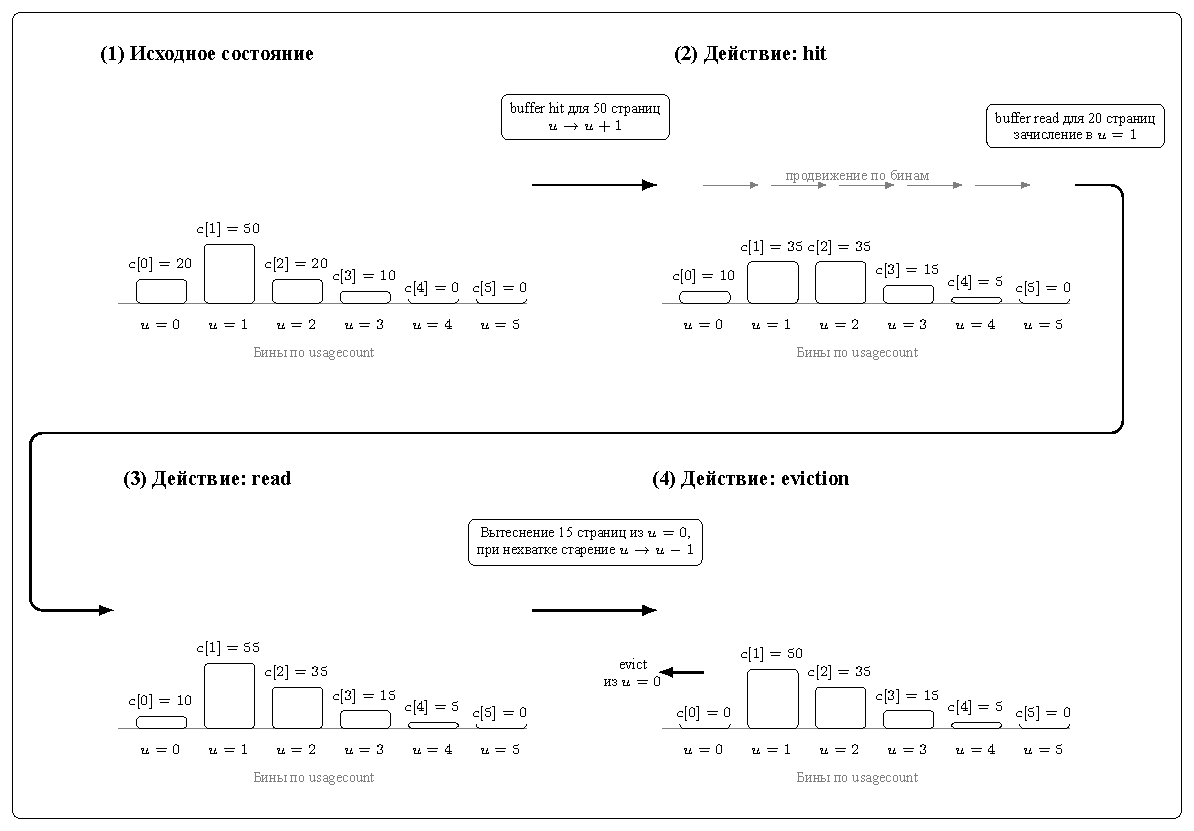
\includegraphics[width=0.95\linewidth]{images/acm_bins.pdf}
%  \fbox{\parbox{0.95\linewidth}{\centering PLACEHOLDER: Бины уровней защищённости и переходы страниц между бинами при обращениях и старении}}
  \caption{Агрегированная модель: распределение страниц по бинам защищённости и его эволюция.}
  \label{fig:usage-bins}
\end{figure}

\paragraph{Правила обновления распределения при выполнении запросов.}
Для каждого запроса $q_i$, который обращается к таблице $T$, доступна статистика буферной активности: число обращений к страницам, обслуженных из памяти ($H_i$), и число страниц, которые пришлось дочитать ($R_i$). Эти величины используются как сигналы для обновления распределения $c_T[u]$:
\begin{enumerate}
  \item \textit{Эффект повторного использования.} При обслуживании обращений из памяти часть уже кешированных страниц считается повторно затронутой. В модели это выражается как повышение их защищённости, то есть перевод некоторой доли страниц из бина $u$ в бин $u+1$ с ограничением сверху на $U$. Для сохранения агрегированного характера считается, что затронутые страницы выбираются пропорционально текущему распределению по бинам.
  \item \textit{Эффект подкачки новых данных.} При появлении страниц, дочитанных с диска, в модели увеличивается число страниц таблицы в низком уровне защищённости, так как такие страницы являются ``слабо защищёнными'' сразу после появления в буфере. Соответственно, часть объёма $R_i$ добавляется в бин $u=1$.
  \item \textit{Ограничение физическим размером таблицы.} Поскольку наблюдаемая статистика учитывает обращения к страницам и может включать повторные обращения к одним и тем же страницам, модель дополнительно ограничивает суммарное число кешированных страниц таблицы $C_T$ сверху её физическим размером $P_T$. В случае превышения распределение $c_T[u]$ пропорционально нормируется так, чтобы $\sum_u c_T[u] \le P_T$.
  \item \textit{Вытеснение при переполнении буфера.} Если суммарное число страниц, предсказанных моделью во всех таблицах, превышает объём буферного пула $B$, выполняется вытеснение. Вытеснение моделируется в два этапа: сначала удаляются страницы из бина $u=0$ (наименее защищённые страницы), а если этого недостаточно, происходит ``старение'' страниц, то есть перевод страниц из $u>0$ в $u-1$, после чего вытеснение из $u=0$ повторяется. Такое правило соответствует интуиции, что страницы постепенно теряют защищённость при отсутствии обращений и становятся кандидатами на вытеснение.
\end{enumerate}

Сформулированные правила задают дискретную динамическую систему, которая по последовательности запросов и их буферной статистике порождает оценку $R_T$ для каждой таблицы на каждом шаге нагрузки.

\paragraph{Экспериментальная постановка.}
Для демонстрации работоспособности подхода использовался синтетический эксперимент с двумя таблицами $T_1$ и $T_2$. Нагрузка генерировалась как последовательность запросов, где на каждом шаге выбиралась одна из таблиц с заданной вероятностью, а объём доступа изменялся случайным образом. Для обеспечения контролируемости и для исключения сценариев, в которых каждый запрос последовательно сканирует всю таблицу, все обращения к таблицам выполнялись с использованием индексных сканирований по диапазону значений ключа. Это позволяет моделировать ситуацию, в которой запросы обращаются к различным частям таблиц и создают переменный объём чтения, что по смыслу близко к работе с несколькими отношениями разного размера и разной интенсивности доступа.

В ходе эксперимента на каждом шаге:
\begin{enumerate}
  \item выполнялся запрос к $T_1$ или $T_2$ с индексным сканированием и случайной шириной диапазона;
  \item фиксировались значения $H_i$ и $R_i$;
  \item обновлялись распределения $c_{T_1}[u]$ и $c_{T_2}[u]$, после чего вычислялись оценки $\widehat{R}_{T_1}$ и $\widehat{R}_{T_2}$.
\end{enumerate}
Для верификации качества прогноза периодически выполнялось контрольное измерение фактической доли страниц таблиц в буферном пуле, после чего оценивались ошибки прогноза.

% PLACEHOLDER FIGURE 3: pred vs truth для t1 и t2, две кривые на графике
\begin{figure}[t]
  \centering
  % \includegraphics[width=0.95\linewidth]{figures/pred_vs_truth_two_tables.pdf}
  \fbox{\parbox{0.95\linewidth}{\centering PLACEHOLDER: Сравнение $\widehat{R}_{T_1}, \widehat{R}_{T_2}$ с фактическими значениями на синтетической нагрузке}}
  \caption{Сравнение прогнозируемой и фактической доли страниц таблиц в shared buffers на синтетической нагрузке.}
  \label{fig:pred-vs-truth}
\end{figure}

\paragraph{Обсуждение.}
Предложенная модель не восстанавливает состав буферного пула на уровне конкретных страниц. Она предназначена для получения правдоподобной оценки прогретости таблиц и её изменения во времени, опираясь на доступные сигналы о буферной активности запросов. Агрегирование через уровни защищённости позволяет приблизить влияние повторного использования страниц и вытеснения при ограниченном размере буфера и тем самым использовать оценку $R_T$ как входной сигнал для стоимостных моделей или адаптивных механизмов оптимизации.

Далее, необходимо связать \(R(q_{t+1})\) с \(random\_page\_cost\) таким образом, чтобы при максимальном прогнозном hit ratio значение \(random\_page\_cost\) совпадало с \(seq\_page\_cost\). Следовательно:
\begin{equation}
    \begin{split}
        random\_page\_cost_{new} = random\_page\_cost_{def} \cdot \\ (1 - R(q_{t+1})) +  seq\_page\_cost \cdot R(q_{t+1})
    \end{split}
\end{equation}
где
\begin{itemize}
    \item \(random\_page\_cost_{def}\) - значение по умолчанию для \(random\_page\_cost\),
    \item \(random\_page\_cost_{new}\) - новое значение для \(random\_page\_cost\), которое будет использовано при расчете стоимости сканирования конкретной таблицы.
\end{itemize}

\begin{figure}[ht]
    \centerfloat{
        
\includegraphics[scale=0.45]{disk model.PNG}
    }
    \caption{Архитектура дисковой модели.}
    \label{fig:disk_architecture}
\end{figure}

На рисунке ~\cref{fig:disk_architecture} показана схема получения статистики использования буфера при выполнении запросов. Чем больше страниц таблицы читается из памяти, тем ниже стоимость последующих случайных обращений, поскольку большинство страниц может быть обслужено из буфера. Следовательно, стоимость случайного доступа к странице необходимо корректировать для каждой таблицы данных.

\subsection{CPU параметры}


\begin{figure}[h]
    \centering
    
\includegraphics[scale=0.5]{cpu model.PNG}
    \caption{Архитектура CPU модели}
    \label{fig:cpu-architecture}
\end{figure}

Другие три параметра стандартной стоимостной модели отвечают за операции,
выполняемые процессором: стоимость обработки одного кортежа (tuples cost),
выполнения одной операции (operator cost) и обработки одного кортежа индекса
(index tuple cost). Стандартные значения этих параметров не отражают специфику
различных аппаратных платформ и конфигураций баз данных, что приводит к неточным
оценкам стоимости запросов. Кроме того, стандартная модель не учитывает
особенности стоимости для разных операторов с индивидуальными формулами расчета
стоимости. Предлагаемая система предоставляет метод сбора статистики и
динамической настройки параметров с учетом конфигурации базы данных и аппаратной
платформы отдельно для каждого оператора плана. На рисунке ~\cref{fig:cpu-architecture} показана схема получения статистики использования CPU во время
выполнения запросов.

После выполнения запроса система собирает ключевую статистику исполнения, такую
как время выполнения операторов, число обработанных кортежей в каждом операторе
и другие показатели. Индивидуальная статистика для каждого типа оператора
накапливается отдельно. На основе этих данных минимизируется расхождение между
значениями, выдаваемыми формулами стоимости операторов, и фактическими временами
их выполнения. Целевая функция строится из легковесных линейных моделей, что не
снижает скорость работы базы данных.

Функция параметров стоимости оператора:

\begin{equation}
    \begin{split}
        & F(c_t, c_o, c_i) = c_t \cdot n_t+c_o \cdot n_o + c_i \cdot n_i + s, \\
        & s = c_s \cdot n_s + c_r \cdot n_r
    \end{split}
    \label{eq:to_min}
\end{equation}
где
\begin{itemize}
    \item \(c_t\) - стоимость обработки одного кортежа,
    \item \(n_t\) - число обработанных кортежей,
    \item \(c_o\) - стоимость выполнения одной операции,
    \item \(n_o\) - число выполненных операций,
    \item \(c_i\) - стоимость обработки одного кортежа индекса,
    \item \(n_i\) - число кортежей индекса,
    \item \(s\) -  стоимость последовательных и случайных чтений для узла при параметрах GUC, полученных из дисковой модели.
\end{itemize}

Исходя из формулы функции стоимости, можно построить простую линейную модель:
\begin{equation}
    L(c,x) = x^T c
    \label{eq:model}
\end{equation}
где вектор \(c=(c_t, c_o, c_i, 1)\) представляет параметры модели, а \(x=(n_t, n_o, n_i, s)\) — независимые переменные. Заметим, что \(s\) рассматривается как независимая переменная, поскольку его значение задаётся дисковой моделью.
Рассмотрим выборку наблюдений \(X\) значений переменных, собранных системой в
процессе выполнения запросов:
\begin{equation}
    X=
    \begin{pmatrix}
        n_t^1 & n_o^1 & n_i^1 & s^1\\
        n_t^2 & n_o^2 & n_i^2 & s^2\\
        ... & ... & ... & ... \\
        n_t^n & n_o^n & n_i^n & s^n\\
    \end{pmatrix}
\end{equation}
Тогда модель \ref{eq:model} можно переписать в матричном виде:
\begin{equation}
    L(c,X) = Xc
    \label{eq:model_matrix}
\end{equation}

Таким образом, задача нахождения оптимальных параметров стоимости сводится к
задаче линейной регрессии:
\begin{equation}
    L(c,X) \rightarrow time \cdot scale\_factor
\end{equation}
где
\begin{itemize}
    \item
    \(time=
    \begin{pmatrix}
        t^1\\
        t^2\\
        ...\\
        t^n\\
    \end{pmatrix}
    \) — собранные времена выполнения оператора,
    \item \(scale\_factor\) — константа, представляющая коэффициент масштабирования
    между временем выполнения и стоимостью.
\end{itemize}
Для оценки параметров модели можно использовать различные методы. В данной работе
использован классический метод наименьших квадратов.

Таким образом, описанная выше процедура позволяет получать точные оценки
параметров стоимости для каждого оператора и устранять ошибки, связанные с
использованием одинаковых параметров стоимости для всех типов операторов.

После сбора статистики и вычисления параметров стоимости система сохраняет
результаты для последующего использования при прогнозировании параметров стоимости
для будущих запросов. При динамической подстройке параметров важно своевременно
реагировать на изменения конфигурации базы данных и другие факторы, влияющие на
стоимости. Поэтому для оперативной реакции на такие изменения система применяет
методы анализа временных рядов для оценки будущих параметров стоимости, когда они
настраиваются индивидуально для каждого типа оператора.
Например, для параметра \(cpu\_tuple\_cost\), предсказанного для моментов времени
\(t_0,..t_{n-1}\): [\(cpu\_tuple\_cost_0\), ..., \(cpu\_tuple\_cost_{n-1}\)],
предсказывается \(cpu\_tuple\_cost_n\) с использованием моделей прогнозирования
временных рядов (например, ARIMA и т. п.). В данной работе использовано
экспоненциальное скользящее среднее:
\begin{equation}
    c_{pred, n} = (1 - \alpha) \cdot c_{n-1} + \alpha \cdot c_{pred, n - 1}
\end{equation}
где
\begin{itemize}
    \item \(c_{pred, i}\) — предсказанное значение параметра стоимости на шаге \(i\),
    \item \(c_i\) — значение параметра стоимости, полученное из линейной модели
    (\ref{eq:model_matrix}) на шаге \(i\),
    \item \(\alpha\) — коэффициент сглаживания.
\end{itemize}

В целом система использует статистику выполнения запросов для калибровки пяти
параметров стоимости, что позволяет планировщику точнее оценивать стоимость для
каждого задействованного типа оператора. Информация для системы включает,
помимо прочего, данные о состоянии буфера, время выполнения запроса и его узлов,
число произведённых кортежей и другие ключевые характеристики.



\section{Тестирование и анализ результатов}\label{sec:ch2/sec3}

\subsection{Тестирование модели прогретости таблиц}


Теперь представим результаты экспериментального тестирования ACM. Возросла ли корреляция между временем и стоимостью для узлов? Улучшилась ли эффективность выполнения бенчмарка? Чтобы ответить на эти вопросы, необходимо рассматривать не только итоговые результаты по времени выполнения, но и величину корреляции между временем и стоимостью для узлов.

ACM тестировалась на двух бенчмарках. Первый это сгенерированный набор данных TPC-H, состоящем из 22 запросов, созданных по шаблонам. Объём сгенерированных данных составил 10 ГБ. Второй бенчмарк JOB (Join Order benchmark). Состоящий из 113 вручную созданных запросов на основе базы данных с информацией о фильмах под названием IMDB. На бенчмарке JOB также было протестирован широко использующийся подход состоящий из калибровочных запросов для оптимизации параметров стоимостной модели.

ACM была реализована в открытой СУБД openGauss, использующей модель стоимости, сходную с PostgreSQL. Для тестирования было выставлено значение shared\_buffers = 16 GB, что позволяет вместить весь набор данных в буфер базы данных. Таким образом время выполнения плана запроса будет больше всего зависеть от выбранного плана, а не от состояния кеша. Также параметр отвечающий за параллельное исполнение запроса был отключен, так чтобы запрос исполнялся в 1 поток, для лучшего контроля за качеством плана. Для обоих датасетов запросы единожны исполнялись для разогрева буферного кеша и сбора статистики по узлам. 

\subsection{Бенчмарк TPC-H}

Для сбора статистики бенчмарк запуска единоразово, после включения прогнозирования параметров каждый запрос запускался 3 раза и бралось медианное значение. Коэффициент сглаживания был выбран 0.2. Размер scale\_factor подбирался из собранной статистики запросов во время сбора метрик.

Рассмотрим корреляцию между стоимостью и временем до применения ACM (рис.\ref{fig:corr_before}) и после (рис.\ref{fig:corr_after}). На рис.~\ref{fig:corr_before} заметны две группы узлов: первая — со временем до 200 мс и значениями стоимости до 5000; вторая — существенно выше, со стоимостью 20 000–25 000 и временем 200–400 мс. Корреляция между стоимостью и временем составляет 0{,}29.
\begin{figure}[h]
\centering

\includegraphics[scale=0.5]{corr before.PNG}
\caption{Корреляция между стоимостью узла и временем выполнения без ACM}
\label{fig:corr_before}
\end{figure}

На рис.~\ref{fig:corr_after} видно, что после применения ACM корреляция усилилась. Крреляция составила 0{,}92. Это указывает на то, что планировщик, используя корректированные параметры модели стоимости, способен улучшать её предсказательную способность.

\begin{figure}[h]
\centering

\includegraphics[scale=0.5]{corr after.PNG}
\caption{Корреляция между стоимостью узла и временем выполнения с ACM}
\label{fig:corr_after}
\end{figure}

На рис.\ref{fig:tpch_results} представлены результаты выполнения бенчмарка TPC-H. Изменение плана наблюдается для запросов 3, 5, 7, 9, 10, 12 и 17. Для остальных запросов план выполнения остался прежним. Совокупное ускорение запросов с модифицированным планом составило 46\%. Ускорение по всему бенчмарку — 20\%. Полные результаты бенчмарка приведены в табл.\ref{tab:results_acm_tpch} в Приложении~\ref{app:A}.

Часть запросов не была оптимизирована после применения ACM. Причиной являются ошибки в оценке кардинальности. Несмотря на повышение корреляции и улучшение модели стоимости, из-за некорректной оценки кардинальностей возможны ошибки. Их следует снижать за счёт методов корректировки оценки кардинальности.

\begin{figure}[h]
\centering

\includegraphics[scale=0.4]{tpch.png}
\caption{Сравнения времен выполнения запросов на бенчмарке TPC-H}
\label{fig:tpch_results}
\end{figure}


\subsection{Бенчмарк JOB и сравнение с конкурентами}

Было проведено сравнение метода ACM с методом калибровочных запросов на бенчмарке JOB.Также как в предыдущем бенчмарке сначала он запускался для сбора статистики и далее каждый запрос запускался 3 раза после чего бралось медианное время выполнения. 


В таблице \ref{tab:job-cost-time-corr} показано изменения корреляций Пирсона и Спирмена на узлах соединений и узлах сканирования при применении калибровочной модели и ACM в сравнении со стандартной стоимостной моделью. Корреляция Спирмена почти не изменилась для обоих моделей, когда корреляция Пирсона возросла с 0.16 до 0.31 и 0.45, соответственно. В таблице \ref{tab:job-runtime-stats} показана статистика времени исполнения бенчмарка. Суммарное время сократилось на 18.49 \% и 23.01 \% для Калибровочной модели стоимости и ACM, соответственно. Стоит упомянуть, что для калибровки параметров стоимостной модели использовались синтетические запросы не входящие в реальную рабочую нагрузку и добавляющие дополнительное время к бенчмарку, которое не учитывается в таблице и составляющее N секунд. В свою очередь ACM способно собрать статистику и начать работать на основе исполнения рабочей нагрузки.  

\begin{table}[h]
\centering
\caption{Корреляция оценки стоимости узлов и фактического времени выполнения на бенчмарке JOB}
\label{tab:job-cost-time-corr}
\begin{tblr}{
  width=\textwidth,
  colspec={X[2,l] Q[r] Q[r] Q[r]},
  row{1}={font=\bfseries},
  hline{1,2,Z} = {solid},
}
Метрика корреляции
  & {Стандартная\\модель стоимости}
  & {Калиброванная\\модель стоимости}
  & {ACM} \\
Спирмен, соединения    & 0.62 & 0.60 & 0.60 \\
Спирмен, сканирования  & 0.80 & 0.85 & 0.86 \\
Спирмен, все операторы & 0.91 & 0.89 & 0.91 \\
Пирсон, соединения     & 0.11 & 0.28 & 0.40 \\
Пирсон, сканирования   & 0.77 & 0.83 & 0.84 \\
Пирсон, все операторы  & 0.16 & 0.31 & 0.45 \\
\end{tblr}
\end{table}

\begin{table}[h]
\centering
\caption{Сводная статистика времени выполнения запросов на бенчмарке JOB}
\label{tab:job-runtime-stats}

\begin{tblr}{
  width=\textwidth,
  colspec={X[2,l] Q[r] Q[r] Q[r]},
  row{1}={font=\bfseries},
  hline{1,2,Z} = {solid},
}
Показатель времени
  & {Стандартная\\модель стоимости}
  & {Калиброванная\\модель стоимости}
  & {ACM} \\
Среднее время, мс                 & 1101   & 897    & 848   \\
Медиана, мс                       & 214    & 198    & 188   \\
95-й перцентиль, мс               & 3871   & 4020   & 3780  \\
Суммарное время бенчмарка, мс     & 124475 & 101460 & 95836 \\
Ускорение по суммарному времени, \% & 0.00 & 18.49 & 23.01 \\
\end{tblr}
\end{table}


\subsection{Выводы}

В данной главе представлена система оперативной онлайн-настройки параметров стоимостной модели на основе телеметрии боевых запросов. Архитектура включает два компонента: модель CPU, корректирующую коэффициенты вычислительных издержек, и модель I/O параметров, использующую сведения о состоянии буферного кэша для уточнения параметров чтения страниц из памяти и с диска. Настройка выполняется в рабочем контуре — без выделения калибровочного трафика и без остановки сервиса. Сохраняется интерпретируемая структура классической стоимостной модели планировщика: изменяются лишь весовые коэффициенты, сама архитектура оптимизатора и порядок перебора планов не затрагиваются. Долгое обучение не требуется — достаточно накопления статистики рабочей нагрузки. Модель постоянно реагирует на изменения нагрузки, в том числе косвенно: при росте общей загруженности сервера корректируются эффективные CPU-параметры. Эксперименты на TPC-H показали, что такая калибровка существенно улучшает согласованность «стоимость–время», а учёт состояния буферов является необходимым условием для корректной интерпретации стоимости операций. Полученные результаты подтверждают целесообразность интеграции адаптивной настройки в контур оптимизатора и демонстрируют потенциал дальнейшего снижения времени исполнения за счёт совместного учёта вычислительных и I/O-характеристик.

Есть и ограничения. Модель не улучшает оценки кардинальностей — эта задача не была в фокусе главы. Для надёжной настройки требуется достаточное представительство операторов в рабочей нагрузке; при наличии единичных наблюдений возможна неустойчивость оценок. Это решается простым ограничением на минимальный объем датасета — начинать обновления только после накопления минимального объёма данных по каждому оператору и применять пороговые проверки перед фиксацией новых коэффициентов. В остальном подход совместим с текущим планировщиком и может быть включён без изменений его архитектуры.

\FloatBarrier
